%----------------------------------------------------------------------------------------
%	PACKAGES AND OTHER DOCUMENT CONFIGURATIONS
%----------------------------------------------------------------------------------------

\documentclass[
		oneside,titlepage,numbers=noenddot,headinclude,%1headlines,
	 	footinclude=true,cleardoublepage=empty,
		dottedtoc, % Make page numbers in the table of contents flushed right with dots leading to them
		BCOR=5mm,paper=a4,fontsize=12pt, % Binding correction, paper type and font size
		italian,american, % Languages, change this to your language(s)
		]{scrreprt} 
                
% Includes the file which contains all the document configurations and packages - make sure to edit this file
%%%%%%%%%%%%%%%%%%%%%%%%%%%%%%%%%%%%%%%%%
% Classicthesis Typographic Thesis
% Configuration File
%
% This file has been downloaded from:
% http://www.LaTeXTemplates.com
%
% Original author:
% André Miede (http://www.miede.de) with extensive commenting changes by:
% Vel (vel@LaTeXTemplates.com)
%
% License:
% GNU General Public License (v2)
%
% Important note:
% The main lines to change in this file are in the DOCUMENT VARIABLES
% section, the rest of the file is for advanced configuration.
%
%%%%%%%%%%%%%%%%%%%%%%%%%%%%%%%%%%%%%%%%%

%----------------------------------------------------------------------------------------
%	CHARACTER ENCODING
%----------------------------------------------------------------------------------------

\PassOptionsToPackage{utf8}{inputenc}
\usepackage{inputenc}
\usepackage{array}
\usepackage{color}
\usepackage{colortbl}
\usepackage{multirow}
\definecolor{flamingopink}{rgb}{0.99, 0.56, 0.67}
\definecolor{icterine}{rgb}{0.99, 0.97, 0.37}
\definecolor{inchworm}{rgb}{0.7, 0.93, 0.36}
%----------------------------------------------------------------------------------------
%	DOCUMENT VARIABLES
%	Fill in the lines below to enter your information into the thesis template
%	Each of the commands can be cited anywhere in the thesis
%----------------------------------------------------------------------------------------

% Remove drafting to get rid of the '[ Date - classicthesis version 4.0 ]' text at the bottom of every page
\PassOptionsToPackage{eulerchapternumbers,listings, pdfspacing, subfig,beramono,eulermath,parts}{classicthesis}
% Available options: drafting parts nochapters linedheaders eulerchapternumbers beramono eulermath pdfspacing minionprospacing tocaligned dottedtoc manychapters listings floatperchapter subfig

\newcommand{\myTitle}{VxWorks 6.9 on Altera Cyclone V  and ZedBoard.
Linux debug on Altera Cyclone V
\xspace}
\newcommand{\mySubtitle}{An Homage to The Elements of Typographic Style\xspace}
\newcommand{\myDegree}{Doktor-Ingenieur (Dr.-Ing.)\xspace}
\newcommand{\myName}{André Miede\xspace}
\newcommand{\myProf}{Put name here\xspace}
\newcommand{\myOtherProf}{Put name here\xspace}
\newcommand{\mySupervisor}{Put name here\xspace}
\newcommand{\myFaculty}{Put data here\xspace}
\newcommand{\myDepartment}{Put data here\xspace}
\newcommand{\myUni}{Put data here\xspace}
\newcommand{\myLocation}{Saarbrücken\xspace}
\newcommand{\myTime}{September 2015\xspace}
\newcommand{\myVersion}{version 4.2\xspace}

%----------------------------------------------------------------------------------------
%	USEFUL COMMANDS
%----------------------------------------------------------------------------------------

\newcommand{\ie}{i.\,e.}
\newcommand{\Ie}{I.\,e.}
\newcommand{\eg}{e.\,g.}
\newcommand{\Eg}{E.\,g.} 

\newcounter{dummy} % Necessary for correct hyperlinks (to index, bib, etc.)
\providecommand{\mLyX}{L\kern-.1667em\lower.25em\hbox{Y}\kern-.125emX\@}
\newlength{\abcd} % for ab..z string length calculation

%----------------------------------------------------------------------------------------
%	PACKAGES
%----------------------------------------------------------------------------------------

\usepackage{lipsum} % Used for inserting dummy 'Lorem ipsum' text into the template


%------------------------------------------------

% Package to generate and customize Algorithm as per ACM style
\usepackage[linesnumbered,commentsnumbered,ruled]{algorithm2e}
\usepackage[italian]{babel}
\usepackage{color}
%------------------------------------------------

%\PassOptionsToPackage{ngerman,american}{babel}  % Change this to your language(s)
% Spanish languages need extra options in order to work with this template
%\PassOptionsToPackage{spanish,es-lcroman}{babel}
%\usepackage{babel}

%------------------------------------------------			

\usepackage{csquotes}
\PassOptionsToPackage{%
%backend=biber, % Instead of bibtex
backend=bibtex8,bibencoding=ascii,%
language=auto,%
style=numeric-comp,%
%style=authoryear-comp, % Author 1999, 2010
%bibstyle=authoryear,dashed=false, % dashed: substitute rep. author with ---
sorting=nyt, % name, year, title
maxbibnames=10, % default: 3, et al.
%backref=true,%
natbib=true % natbib compatibility mode (\citep and \citet still work)
}{biblatex}
\usepackage{biblatex}
\usepackage{ragged2e}
 %------------------------------------------------

\PassOptionsToPackage{fleqn}{amsmath} % Math environments and more by the AMS 
 \usepackage{amsmath}
 
 %------------------------------------------------

\PassOptionsToPackage{T1}{fontenc} % T2A for cyrillics
\usepackage{fontenc}

%------------------------------------------------

\usepackage{textcomp} % Fix warning with missing font shapes

%------------------------------------------------

\usepackage{scrhack} % Fix warnings when using KOMA with listings package  

%------------------------------------------------

\usepackage{xspace} % To get the spacing after macros right

%------------------------------------------------

\usepackage{mparhack} % To get marginpar right

%------------------------------------------------

\usepackage{fixltx2e} % Fixes some LaTeX stuff 

%------------------------------------------------

\PassOptionsToPackage{smaller}{acronym} % Include printonlyused in the first bracket to only show acronyms used in the text
\usepackage{acronym} % Nice macros for handling all acronyms in the thesis

%\renewcommand*{\acsfont}[1]{\textssc{#1}} % For MinionPro
\renewcommand*{\aclabelfont}[1]{\acsfont{#1}}

%------------------------------------------------

\PassOptionsToPackage{pdftex}{graphicx}
\usepackage{graphicx} 

%----------------------------------------------------------------------------------------
%	FLOATS: TABLES, FIGURES AND CAPTIONS SETUP
%----------------------------------------------------------------------------------------

\usepackage{tabularx} % Better tables
\setlength{\extrarowheight}{3pt} % Increase table row height
\newcommand{\tableheadline}[1]{\multicolumn{1}{c}{\spacedlowsmallcaps{#1}}}
\newcommand{\myfloatalign}{\centering} % To be used with each float for alignment
\usepackage{caption}
\captionsetup{font=small}
\usepackage{subfig}  

%----------------------------------------------------------------------------------------
%	CODE LISTINGS SETUP
%----------------------------------------------------------------------------------------
\usepackage{color}
 
\usepackage[dvipsnames]{xcolor}

\definecolor{keywords}{RGB}{255, 255, 255}
\definecolor{cobalt}{rgb}{0.0, 0.28, 0.67}
\definecolor{darkgray}{rgb}{0.66, 0.66, 0.66}
 
\definecolor{codegreen}{rgb}{0,0.6,0}
\definecolor{codegray}{rgb}{0.5,0.5,0.5}
\definecolor{codepurple}{rgb}{0.58,0,0.82}
\definecolor{backcolour}{rgb}{0.95,0.95,0.92}


\usepackage{listings,lstautogobble} 
%\lstset{emph={trueIndex,root},emphstyle=\color{BlueViolet}}%\underbar} % For special keywords

\lstloadlanguages{SQL} % load java, needed because of option 'savemem'

\lstdefinestyle{myCode}{
texcl=true,
%language=SQL,%C++ % Specify the language(s) for listings here
%keywordstyle=\color{RoyalBlue}, % Add \bfseries for bold
%keywordstyle=\color{black},
keywordstyle=[2]\color{cobalt},
keywordstyle=[3]\color{RoyalBlue}, 
keywordstyle=[4]\color{orange},
keywordstyle=[5]\color{yellow},
basicstyle=\scriptsize\ttfamily, % Makes listings a smaller font size and a different font
%identifierstyle=\color{NavyBlue}, % Color of text inside brackets
commentstyle=\color{darkgray}\ttfamily, % Color of comments
morecomment=[l]{--}, % l is for line comment
morecomment=[s]{/*}{*/}, % s is for start and end delimiter
stringstyle=\rmfamily, % Font type to use for strings
numbers=left, % Change left to none to remove line numbers
numberstyle=\scriptsize, % Font size of the line numbers
stepnumber=1, % Increment of line numbers
numbersep=8pt, % Distance of line numbers from code listing
showstringspaces=false, % Sets whether spaces in strings should appear underlined
breaklines=true, % Force the code to stay in the confines of the listing box
%frameround=ftff, % Uncomment for rounded frame
%frame=single, % Frame border - none/leftline/topline/bottomline/lines/single/shadowbox/L
tabsize=2,
autogobble=true,
belowcaptionskip=.75\baselineskip, % Space after the "Listing #: Desciption" text and the listing box
keywords=[2]{define},
keywords=[3]{},
keywords=[4]{bootloader, bin}
 }

%----------------------------------------------------------------------------------------
%	HYPERREFERENCES
%----------------------------------------------------------------------------------------

\PassOptionsToPackage{pdftex,hyperfootnotes=false,pdfpagelabels}{hyperref}
\usepackage{hyperref}  % backref linktocpage pagebackref
\pdfcompresslevel=9
\pdfadjustspacing=1



\hypersetup{
% Uncomment the line below to remove all links (to references, figures, tables, etc), useful for b/w printouts
%draft, 
colorlinks=true, linktocpage=true, pdfstartpage=3, pdfstartview=FitV,
% Uncomment the line below if you want to have black links (e.g. for printing black and white)
%colorlinks=false, linktocpage=false, pdfborder={0 0 0}, pdfstartpage=3, pdfstartview=FitV, 
breaklinks=true, pdfpagemode=UseNone, pageanchor=true, pdfpagemode=UseOutlines,%
plainpages=false, bookmarksnumbered, bookmarksopen=true, bookmarksopenlevel=1,%
hypertexnames=true, pdfhighlight=/O,%nesting=true,%frenchlinks,%
urlcolor=RoyalBlue, linkcolor=RoyalBlue, citecolor=webgreen, %pagecolor=RoyalBlue,%
    %urlcolor=Black, linkcolor=Black, citecolor=Black, %pagecolor=Black,%
%------------------------------------------------
% PDF file meta-information
pdftitle={\myTitle},
pdfauthor={\textcopyright\ \myName, \myUni, \myFaculty},
pdfsubject={},
pdfkeywords={},
pdfcreator={pdfLaTeX},
pdfproducer={LaTeX with hyperref and classicthesis}
%------------------------------------------------
}

%----------------------------------------------------------------------------------------
%	AUTOREFERENCES SETUP
%	Redefines how references in text are prefaced for different 
%	languages (e.g. "Section 1.2" or "section 1.2")
%----------------------------------------------------------------------------------------

\makeatletter
\@ifpackageloaded{babel}
{
\addto\extrasamerican{
\renewcommand*{\figureautorefname}{Figure}
\renewcommand*{\tableautorefname}{Table}
\renewcommand*{\partautorefname}{Part}
\renewcommand*{\chapterautorefname}{Chapter}
\renewcommand*{\sectionautorefname}{Section}
\renewcommand*{\subsectionautorefname}{Section}
\renewcommand*{\subsubsectionautorefname}{Section}
}
\addto\extrasngerman{
\renewcommand*{\paragraphautorefname}{Absatz}
\renewcommand*{\subparagraphautorefname}{Unterabsatz}
\renewcommand*{\footnoteautorefname}{Fu\"snote}
\renewcommand*{\FancyVerbLineautorefname}{Zeile}
\renewcommand*{\theoremautorefname}{Theorem}
\renewcommand*{\appendixautorefname}{Anhang}
\renewcommand*{\equationautorefname}{Gleichung}
\renewcommand*{\itemautorefname}{Punkt}
}
\providecommand{\subfigureautorefname}{\figureautorefname} % Fix to getting autorefs for subfigures right
}{\relax}
\makeatother

%----------------------------------------------------------------------------------------

\usepackage{classicthesis} 

%----------------------------------------------------------------------------------------
%	CHANGING TEXT AREA 
%----------------------------------------------------------------------------------------

%per ampliare i margini decommentare la seguente linea ma fare attenzione perchè incasina il posizionamento di alcune immagini 
\usepackage[a4paper,top=3cm,bottom=3.5cm,left=2.5cm,right=2.5cm]{geometry}

%\linespread{1.05} % a bit more for Palatino
%\areaset[current]{312pt}{761pt} % 686 (factor 2.2) + 33 head + 42 head \the\footskip
%\setlength{\marginparwidth}{em}%
%\setlength{\marginparsep}{2em}%

%----------------------------------------------------------------------------------------
%	USING DIFFERENT FONTS
%----------------------------------------------------------------------------------------

%\usepackage[oldstylenums]{kpfonts} % oldstyle notextcomp
%\usepackage[osf]{libertine}
%\usepackage[light,condensed,math]{iwona}
%\renewcommand{\sfdefault}{iwona}
%\usepackage{lmodern} % <-- no osf support :-(
%\usepackage{cfr-lm} % 
%\usepackage[urw-garamond]{mathdesign} <-- no osf support :-(
%\usepackage[default,osfigures]{opensans} % scale=0.95 
%\usepackage[sfdefault]{FiraSans}

\addbibresource{Bibliography.bib} 
\usepackage{eso-pic}
\usepackage{tikz}
\newcommand\BackgroundPic{%
	\put(0,0){%
		\parbox[b][\paperheight]{\paperwidth}{%
			\vfill
			\centering
			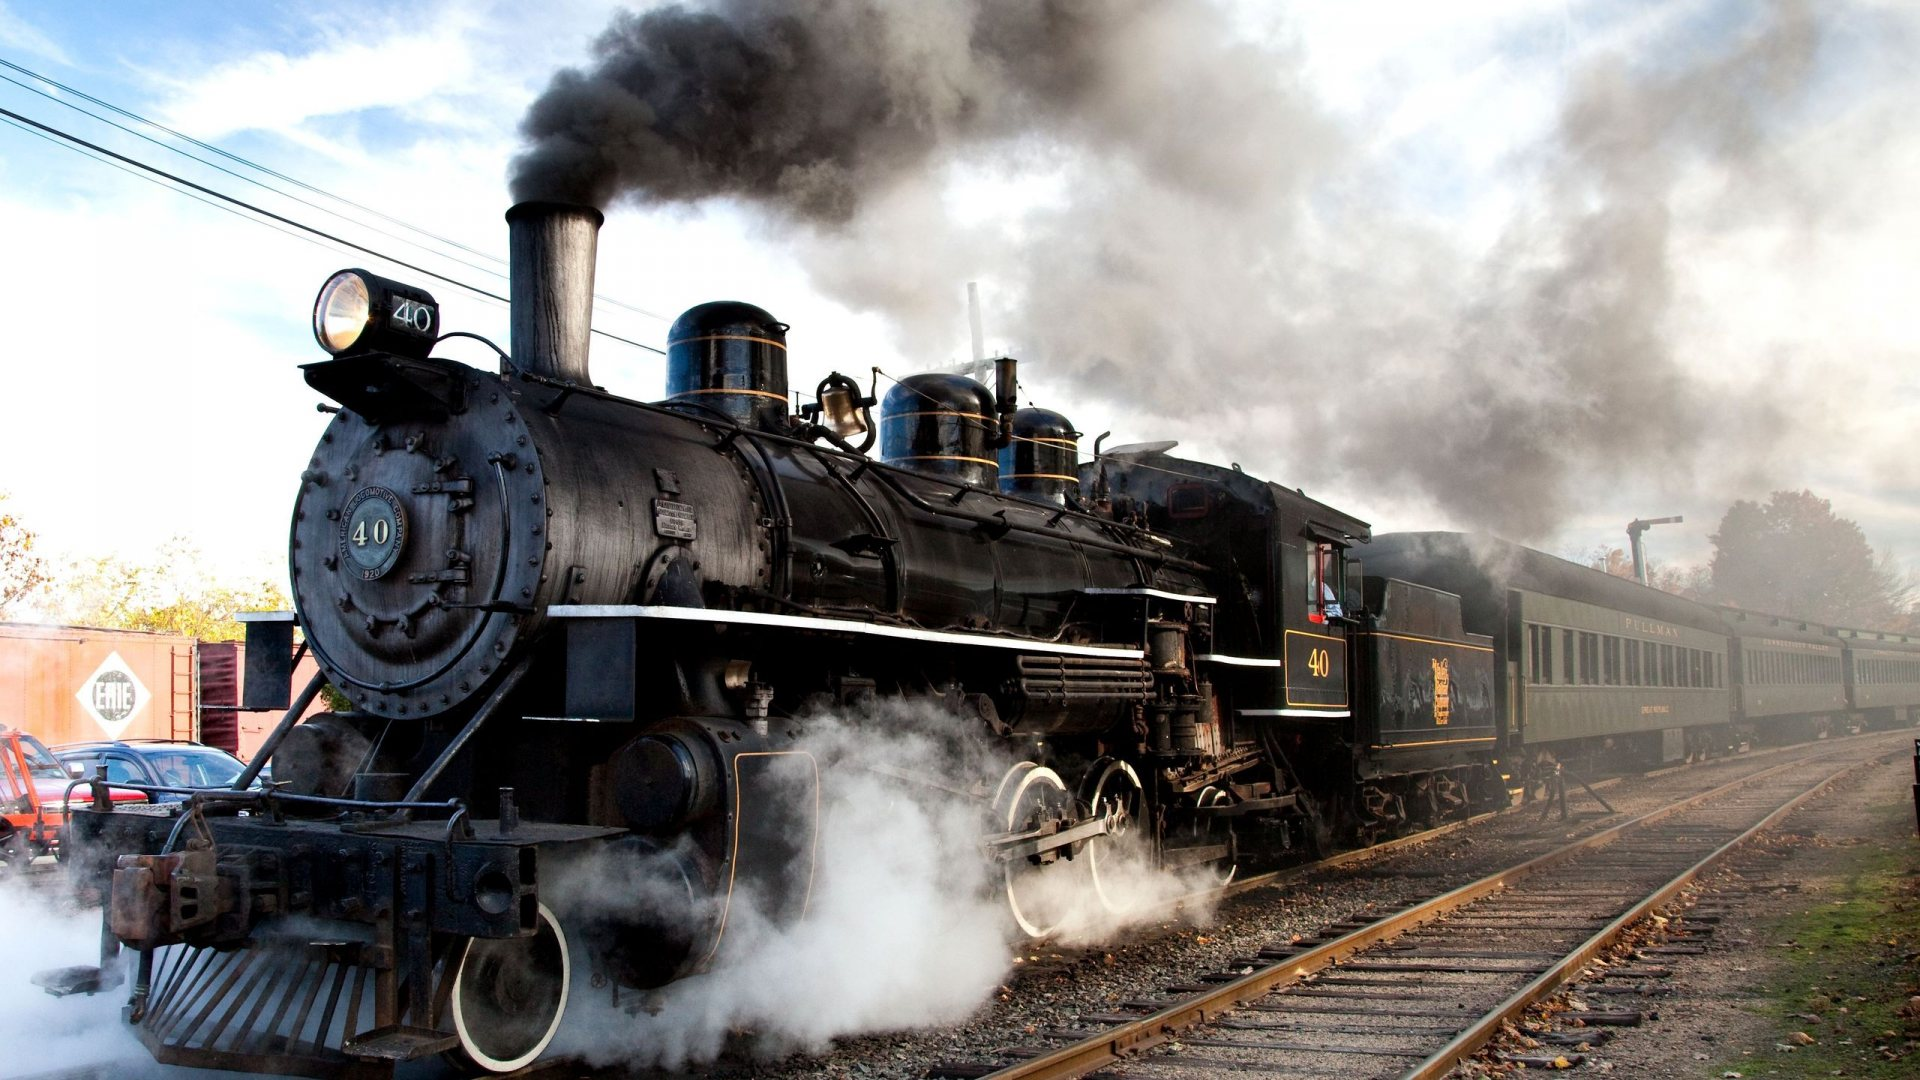
\includegraphics[width=\paperwidth,height=\paperheight,%
			keepaspectratio]{img/train.jpg}%
			\vfill
}}}


\begin{document}

\AddToShipoutPicture*{\BackgroundPic}

\frenchspacing % Reduces space after periods to make text more compact

\raggedbottom % Makes all pages the height of the text on that page

\selectlanguage{italian}

\pagenumbering{roman} % Roman page numbering prior to the start of the thesis content (i, ii, iii, etc)

\pagestyle{plain} % Suppress headers for the pre-content pages

%-------------------------------------------------------------------
%	Frontespizio-Indice
%-------------------------------------------------------------------

% Title Page

\begin{titlepage}




	\begin{center}
		\large
		\centering
		
		\begingroup
		\color{Maroon}\spacedallcaps{VxWorks 6.9 on Altera Cyclone V  and ZedBoard.
Linux debug on Altera Cyclone V
 } \newline
		\color{Maroon}\spacedallcaps{  } \\ \bigskip
		\endgroup

\vfill
\vfill
\vfill
\vfill
\vfill
\vfill
\vfill
\vfill
\vfill
\spacedlowsmallcaps{Mattia Ciolli}
\\
\spacedlowsmallcaps{Matteo Polsinelli}
\\
\spacedlowsmallcaps{Davide Giancola}
\vfill






\end{center}


\end{titlepage} % Main title page
\cleardoublepage
\cleardoublepage% Table of Contents - List of Tables/Figures/Listings and Acronyms

\refstepcounter{dummy}

\pdfbookmark[1]{\contentsname}{tableofcontents} % Bookmark name visible in a PDF viewer

\setcounter{tocdepth}{2} % Depth of sections to include in the table of contents - currently up to subsections

\setcounter{secnumdepth}{3} % Depth of sections to number in the text itself - currently up to subsubsections

\manualmark
\markboth{\spacedlowsmallcaps{\contentsname}}{\spacedlowsmallcaps{\contentsname}}
\tableofcontents 
\automark[section]{chapter}
\renewcommand{\chaptermark}[1]{\markboth{\spacedlowsmallcaps{#1}}{\spacedlowsmallcaps{#1}}}
\renewcommand{\sectionmark}[1]{\markright{\thesection\enspace\spacedlowsmallcaps{#1}}}

\clearpage

\begingroup 
\let\clearpage\relax
\let\cleardoublepage\relax
\let\cleardoublepage\relax

%----------------------------------------------------------------------------------------
%	List of Figures
%----------------------------------------------------------------------------------------

\refstepcounter{dummy}
%\addcontentsline{toc}{chapter}{\listfigurename} % Uncomment if you would like the list of figures to appear in the table of contents
\pdfbookmark[1]{\listfigurename}{lof} % Bookmark name visible in a PDF viewer

\listoffigures

\vspace{8ex}
\newpage
        

 
                   
\endgroup % Contents, list of figures/tables/listings and acronyms

\cleardoublepage

\pagenumbering{arabic} 

\cleardoublepage % Avoids problems with pdfbookmark

%----------------------------------------------------------------------------------------
%	Contenuto della relazione
%----------------------------------------------------------------------------------------

\chapter{Introduction}

\label{ch:introduction}
La mobilità delle persone e delle merci sono una componente essenziale del mercato interno dell'Unione Europea (UE) ed è di fondamentale importanza garantire la sua fattibilità al fine di salvaguardare la crescita economica.
La rete ferroviaria ha un ruolo strategico in questo contesto almeno sotto due punti di vista:

\chapter{Altera Cyclone V VxWorks Boot} % Chapter title

\label{ch:materialandmethods} % For referencing the chapter elsewhere, use \autoref{ch:examples} 

%----------------------------------------------------------------------------------------

\section{Overview}
\label{overview}
The following figure depicts the typical boot flow: \\
\begin{figure}[h]
	\centering		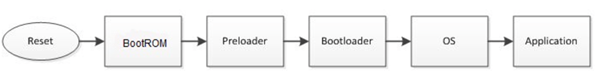
\includegraphics[width=0.8\textwidth]{img/bootschema1}
	\caption{Boot flow}
    	\label{fig:bootflow}
\end{figure}

Additional boot flows are possible, as shown in the following diagram:
\begin{figure}[h]
	\centering		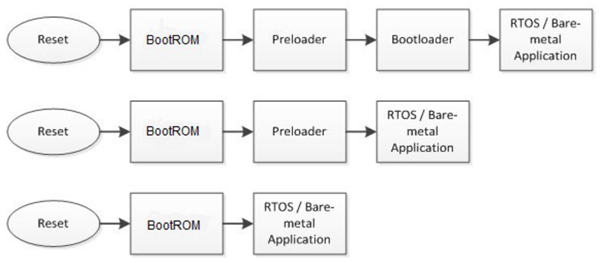
\includegraphics[width=0.8\textwidth]{img/bootschema2}
	\caption{Additional boot flow}
    	\label{fig:bootflow2}
\end{figure}

\textbf{The HPS boot} process starts when the processor is released from reset, and jumps to the reset vector address, located in the Boot ROM address space.\newline
Typically, the main responsibilities of the Boot ROM are: 
\begin{itemize}
\item Detect the selected boot source;
\item Perform minimal HPS initialization; 
\item Load the next boot stage (typically the Preloader) from Flash to OCRAM and jump to it.
\end{itemize}
The behavior of the Boot ROM is influenced by the BSEL and CSEL options (rev B, C).\\
Typical board switches layout found in the references.
\begin{figure}[h]
	\centering		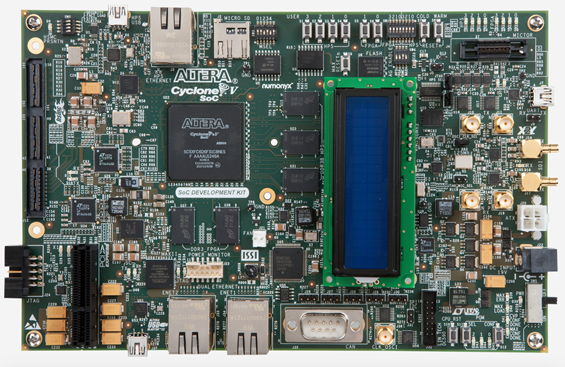
\includegraphics[width=0.8\textwidth]{img/ciclonv1}
	\caption{Altera Cyclon V}
    	\label{fig:ciclonv1}
\end{figure}
\begin{figure}[h]
	\centering		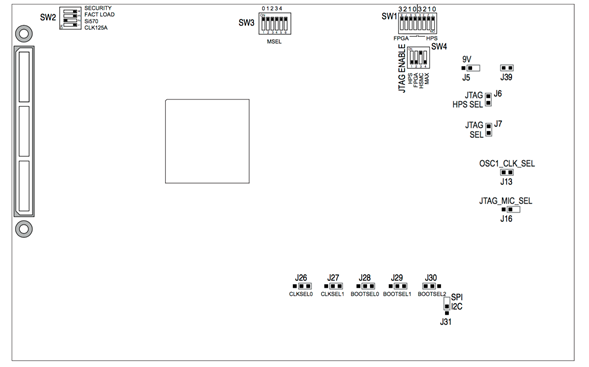
\includegraphics[width=0.8\textwidth]{img/ciclonv2}
	\caption{Altera Cyclon V switchs}
    	\label{fig:ciclonv2}
\end{figure}

\clearpage
\newpage

Our board. The switches are configured for FPGA Working Mode.
\begin{figure}[h]
	\centering		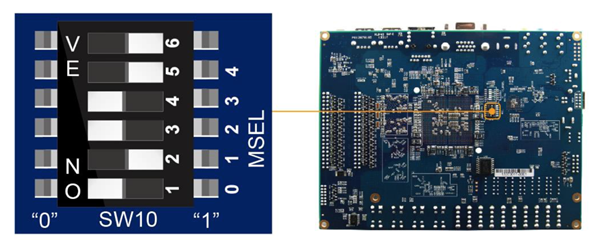
\includegraphics[width=0.8\textwidth]{img/ciclonv3}
	\caption{MSEL}
    	\label{fig:ciclonv3}
\end{figure}


Running Linux to check the correct configuration of the board switches.
\begin{itemize}
\item \textbf{What is necessary:}

\begin{enumerate}
\item SD card ( At least 4 gb);
\item Win32DiskImager.exe ( \url{http://sourceforge.net/projects/win32diskimager/} to flash the Linux Image on the SD; 
\item Pre-built SD Card Image ( \url{http://www.terasic.com/downloads/cd-rom/de1-soc/linux_BSP/DE1_SoC_SD.zip}.);
\item Putty.
\end{enumerate}

\item \textbf{What is inside the default image:}

\begin{enumerate}
\item SPL Pre-loader;
\item U-boot; 
\item Device Tree Blob;
\item Linux Kernel;
\item Linux Root File system.
\end{enumerate}

\item \textbf{MSEL CONFIGURATION}
\begin{figure}[h]
	\centering		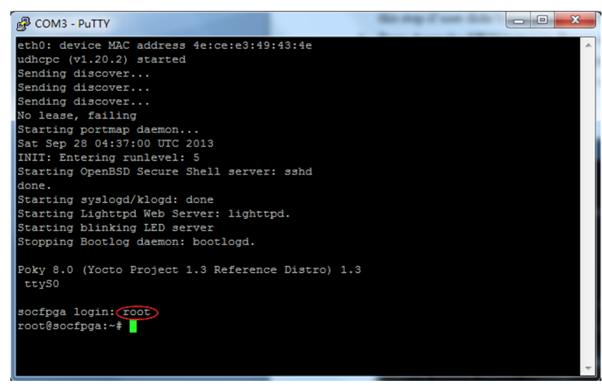
\includegraphics[width=0.8\textwidth]{img/putty1}
	\caption{Shown with Putty application}
    	\label{fig:putty}
\end{figure}
\begin{figure}[h]
	\centering		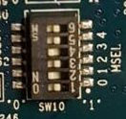
\includegraphics[width=0.3\textwidth]{img/msel}
	\caption{Msel switchs}
    	\label{fig:msel}
\end{figure}
\end{itemize}

\clearpage
\newpage
The preloader configures clocking, IOCSR, pinmuxing, DDRAM and loads the second-stage bootloader( like U-boot  or in our case the VxWorks bootloader ) into DDRAM.

\begin{figure}[h]
	\centering		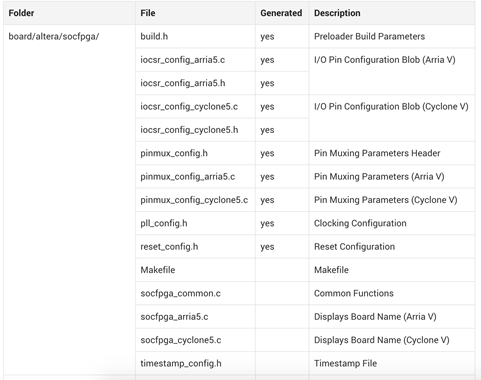
\includegraphics[width=0.8\textwidth]{img/folder}
	\caption{socfpga folder}
    	\label{fig:folder}
\end{figure}

\clearpage
\section{Preloader}
\label{preloader}

\begin{figure}[h]
	\centering		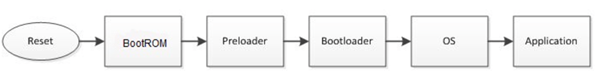
\includegraphics[width=0.8\textwidth]{img/bootschema1}
	\caption{Boot flow}
    	\label{fig:bootflow}
\end{figure}

The modifications made to the uboot-socfpga/board/altera/socfpga/build.h file are shown below in bolded text: 

\begin{lstlisting}[style=myCode]
/* Enable FAT partition support when booting from SDMMC. */ 
#define CONFIG_PRELOADER_FAT_SUPPORT (1)

/* When FAT partition support is enabled, this specifies the * FAT partition where the boot image is located. */
#define CONFIG_PRELOADER_FAT_BOOT_PARTITION (1)

/* When FAT partition supported is enabled, this specifies the * boot image filename within a FAT partition to be used as fatload payload.*/
#define CONFIG_PRELOADER_FAT_LOAD_PAYLOAD_NAME "bootloader.bin" 
\end{lstlisting}   

Another change where the preloader loads the FPGA file was made to the uboot-socfpga/include/configs/ socfpga\_common.h file:

\begin{lstlisting}[style=myCode]
/*  FPGA programming support with SPL FPGA RBF file source (with mkimage header) is located within the same  boot device which stored the subsequent boot image (U-Boot). */

/* enabled program the FPGA */
#define CONFIG_SPL_FPGA_LOAD 
\end{lstlisting} 

\clearpage
\section{Bootloader}
\label{bootloader}

\begin{figure}[h]
	\centering		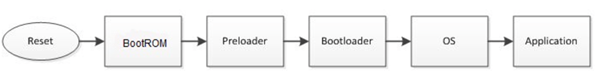
\includegraphics[width=0.8\textwidth]{img/bootschema1}
	\caption{Boot flow}
    	\label{fig:bootflow}
\end{figure}

We have built the  VxWorks bootrom file using Wind River tools and the alt\_soc\_gen5 BSP using the workbench of Wind River.
	
\begin{lstlisting}[style=myCode]
-A arm -T firmware -C none -O vxworks -a 0x08000040 -  e 0 -n "vxWorks bootloader for SoC FPGA" -d bootrom.bin  bootloader.bin 
\end{lstlisting} 

Finally we have put everything on the SD Card and we had tried to boot the system with no results.\\					
This method is described by the official documentation from the Intel/Altera site.  Also the software is provided.
\begin{figure}[h]
	\centering		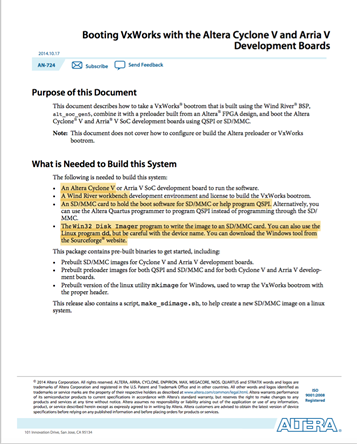
\includegraphics[width=0.6\textwidth]{img/bootguide}
	\caption{Boot cyclonV guide}
    	\label{fig:bootguide}
\end{figure}

\clearpage
\section{From scratch}
\label{Fromscratch}

\begin{figure}[h]
	\centering		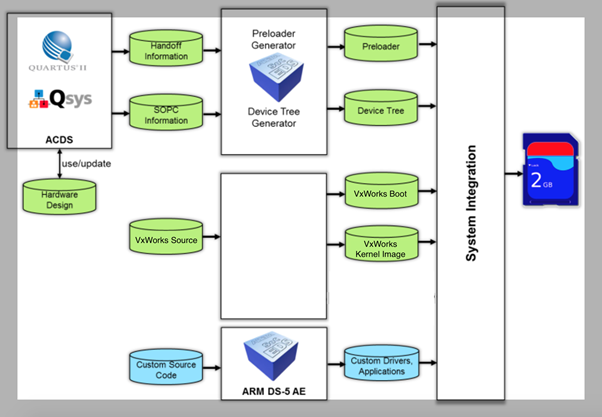
\includegraphics[width=0.6\textwidth]{img/fromscratch}
	\caption{From scratch}
    	\label{fig:fromscratch}
\end{figure}

\subsection{Compiling the Hardware Design}
\begin{figure}[h]
	\centering		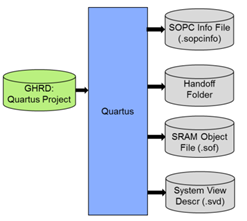
\includegraphics[width=0.4\textwidth]{img/ghrd}
	\caption{GHRD}
    	\label{fig:ghrd}
\end{figure}

\begin{figure}[h]
	\centering		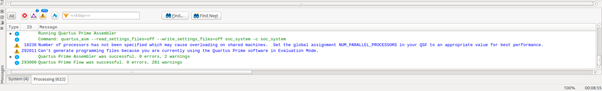
\includegraphics[width=0.8\textwidth]{img/quartuserror}
	\caption{Quartus Error}
    	\label{fig:quartuserror}
\end{figure}


\url{https://rocketboards.org/foswiki/view/Documentation/GSRDCompileHardwareDesign}.

\subsection{Compiling the Preloader}
\begin{figure}[h]
	\centering		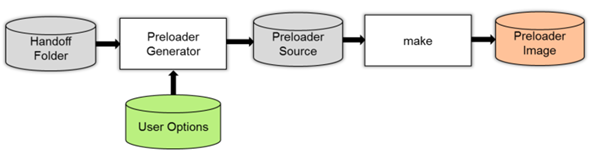
\includegraphics[width=0.8\textwidth]{img/schema}
	\caption{Compiling schema}
    	\label{fig:schema}
\end{figure}

\url{https://rocketboards.org/foswiki/view/Documentation/GSRDPreloader}.

\subsection{Device Tree}
The device tree is a data structure for describing hardware. 
Given the correct device tree, the same compiled kernel can support different hardware configurations within a wider architecture family.\\
For ARM, use of device trees has become mandatory for all new SoCs.\\
This can be seen as a remedy to the vast number of forks (of Linux and Das U-boot) that has historically been created to support (marginally) different ARM boards.\\

\begin{figure}[h]
	\centering		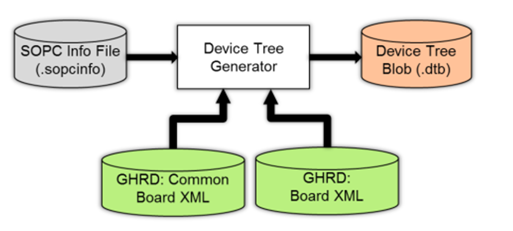
\includegraphics[width=0.6\textwidth]{img/devicetree}
	\caption{Device tree}
    	\label{fig:devicetree}
\end{figure}

\url{https://rocketboards.org/foswiki/view/Documentation/GSRDDeviceTreeGenerator}.

\subsection{Vivado}
We used Vivado on the workstation to build ….
We built the VxWorks image for the Cyclone V.
Building the device tree it gave an error, so we forced the output.\\ 
We put on the SD the image, the device tree and the bootloader.\\
We tried to boot but nothing showed up, neither with the forced device tree, nor with the .dts file already provided.\\

\begin{figure}[h]
	\centering		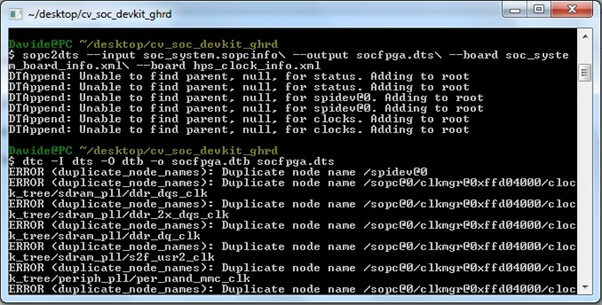
\includegraphics[width=0.6\textwidth]{img/devicetreeerror}
	\caption{Device tree error}
    	\label{fig:devicetreeerror}
\end{figure}






\chapter{Zedboard}
\label{ch:zedboard}

After having failed to boot VxWorks on the Cyclone V and waiting for Quartus licence, we decided to try to boot the same RTOS on the Zedboard, a Zynq-7000 based board.\\
This board was chosen because we have seen that it has official documentation 
and guides and it’s one of the boards supported by VxWorks. \\
Moreover there are programs like Vivado to develop and debug software.

\section{Overview}
\begin{figure}[h]
	\centering		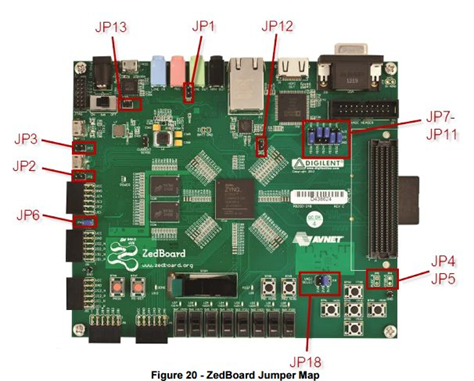
\includegraphics[width=0.8\textwidth]{img/zedboard}
	\caption{Zedboard}
    	\label{fig:zedboard}
\end{figure}

\begin{itemize}
\item SD Card;
\item 512 MB DDR3 (128M x 32) o 256 Mb QSPI Flash;
\item USB 2.0 FS USB-UART bridge;
\item Dual ARM Cortex-A9 MPCore Up to 667 MHz.
\end{itemize}


\section{Building the kernel image}
We have built the kernel image with Windriver workbench following this guide:\\
\href{https://www.xilinx.com/support/documentation/application_notes/xapp1158-zynq-7000-vxworks-bsp.pdf}{Guide}\\
We created the .bif file with the following format:

\begin{lstlisting}[style=myCode]
ZC702_bif_for_VxWorks: 
{ 
[bootloader]zynq_fsbl_0.elf 
bootROM.elf 
}
\end{lstlisting} 
And downloaded the .elf file from the official Xilinx website.

\section{Generating the bootloader}
We built the bootloader using the Vivado TCL shell using “bootgen” following this guide \url{http://www.wiki.xilinx.com/Prepare+boot+image} omitting the “I” parameter  because was not recognised.\\

\begin{figure}[h]
	\centering		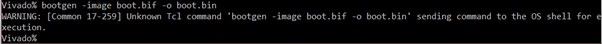
\includegraphics[width=0.8\textwidth]{img/bootloaderbuild}
	\caption{Bootloader build}
    	\label{fig:bootloaderbuild}
\end{figure}

\subsection{Bootloader}
\begin{figure}[h]
	\centering		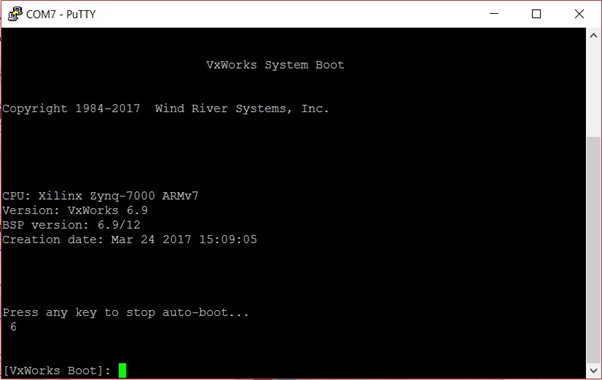
\includegraphics[width=0.6\textwidth]{img/boot}
	\caption{Boot}
    	\label{fig:boot}
\end{figure}

We installed the Cypress drivers for the serial interface.\\
We copied boot.bin e vxWorks on the SD card and connected with Putty. \\
The bootloader started up.

\subsection{Bootloader configuration}
We stopped the autoboot, then we inserted the following instructions as suggested  from the guide:\\
\href{https://www.xilinx.com/support/documentation/application_notes/xapp1158-zynq-7000-vxworks-bsp.pdf}{Guide}

\begin{figure}[h]
	\centering		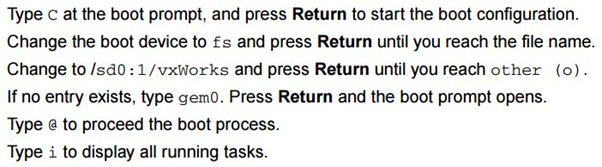
\includegraphics[width=0.8\textwidth]{img/code}
	\caption{Code}
    	\label{fig:code}
\end{figure}

\subsection{Errors and bugs}
After some attempts it gave us the following error\\

\begin{lstlisting}[style=myCode]
Host Name: bootHost
Target Name: vxTarget
User: target
ERROR: ipcom_drv_eth_init: drvname:, drvunit: 0
0x1100e5c (tRootTask): task 0x1100e5c has had a failure and has been stopped.
0x1100e5c (tRootTask): fatal exception in a kernel task or stack overflow!
Instantiating /sd0:0 as rawFs,  device = 0x10001
\end{lstlisting} 

We noticed that the parameters inserted previously are not stored in the SD but in internal memory. So resetting, rebooting, formatting the SD and installing Linux had no effect in deleting those values.

\section{XMD console}
We used the Xilinx SDK (Software development kit), a software installed with Vivado, used to develop embedded applications.\\
We tried to put the bootloader and the image directly in RAM with the XMD console included in the SDK.\\
Trying to connect with the connect command we have discovered that 2 usb cable were needed: the first for the serial, the second connected to the PROG port.

\subsection{Connected to the board}
Following this guide \url{https://www.xilinx.com/support/documentation/sw_manuals/xilinx2014_1/ug1043-embedded-system-tools.pdf} pg.73, we inserted the command “connect arm hwCortexA9” without result.\\
Following the help of the console we discovered that the right command is “connect arm hw”.\\

\begin{figure}[h]
	\centering		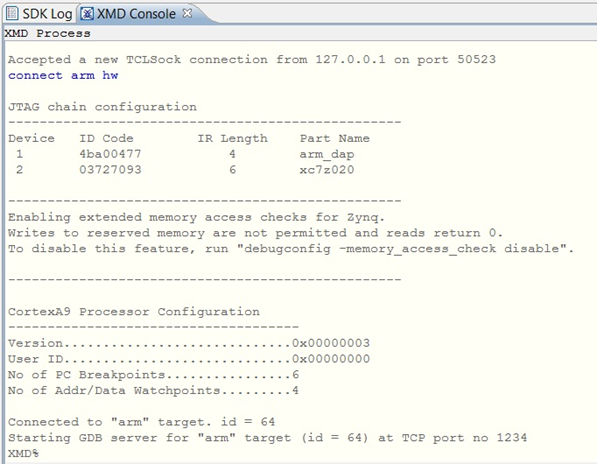
\includegraphics[width=0.6\textwidth]{img/xmdconnect}
	\caption{XMD connect}
    	\label{fig:xmdconnect}
\end{figure}


\subsection{RAM busy}
Once connected we tried to put the files directly in RAM. we executed the command “dow -data boot.bin 0x00100000” giving us the following error:

\begin{lstlisting}[style=myCode]
AP transaction error (DP CTRL_STAT=0xf0000021)
Error Address = 0x00100000, Size = 0x00000004
\end{lstlisting}

We discovered that the problem wasn’t the register but the fact that the processor was not stopped and the memory was busy

\subsection{Missing component}
We tried to manually stop and reset the processor with “stop” and “rst” commands. After some researches we discovered that ps7\_init.tcl was missing. We downloaded it and we used it to stop the processor:


\begin{lstlisting}[style=myCode]
source ps7_init.tcl
ps7_init
ps7_post_config
stop
\end{lstlisting}

\subsection{Directly in RAM}
We were able to stop the processor and to put the files in RAM with the “dow” command. Then we gave the “con”  and “run” command but nothing showed up in Putty. 

\begin{lstlisting}[style=myCode]
XMD% con

RUNNING> XMD%
\end{lstlisting}

After this we asked help on the knowledge forum to resolve the stackoverflow problem but no one was able to help us 
\url{https://ask.windriver.com/en/questions/35789/zedboard-boot-vxworks-69-problem/}.



 



















\chapter{Another zedboard} 
\label{ch:anotherzedboard} 

We changed board and the bootloader started well without giving the stackoverflow error but randomly didn’t start.\\
After having tried the same parameters previously inserted, the bootloader couldn’t  initialize inet and some network settings.

\begin{figure}[h]
	\centering		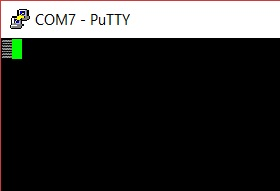
\includegraphics[width=0.6\textwidth]{img/error1}
	\caption{Error}
    	\label{fig:error1}
\end{figure}

\begin{figure}[h]
	\centering		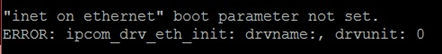
\includegraphics[width=0.6\textwidth]{img/error2}
	\caption{Another error}
    	\label{fig:error2}
\end{figure}

\section{Wrong kernel image}

Following this guide 
\href{https://www.xilinx.com/support/documentation/application_notes/xapp1258-vxworks-7-bsp.pdf}{Guide}
we tried to boot the vxWorks image but it can’t get the kernel image.
\begin{figure}[h]
	\centering		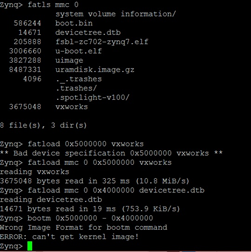
\includegraphics[width=0.4\textwidth]{img/error3}
	\caption{Wrong kernel image}
    	\label{fig:error3}
\end{figure}

\section{U-BOOT}
We rebuilded the image following the configurations parameters provided by the guide  but we had the same error.

\begin{figure}[h]
	\centering		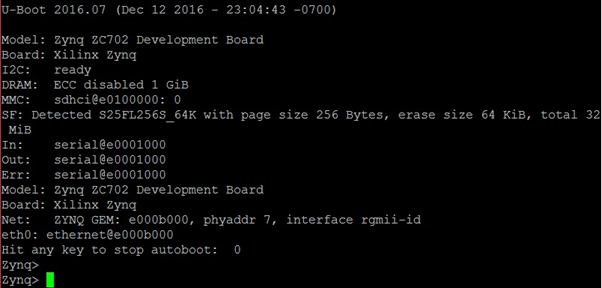
\includegraphics[width=0.6\textwidth]{img/error4}
	\caption{Boot problem}
    	\label{fig:error4}
\end{figure}





\chapter{Linux On Cyclone V}
\label{ch:linuxoncyclonev}

We have downloaded the system image from the Altera website and put it on the SD card with Win32DiskImager.exe.\\
We connected with Putty and it showed that Linux booted up successfully.

\section{Debug on Linux}
\begin{figure}[h]
	\centering		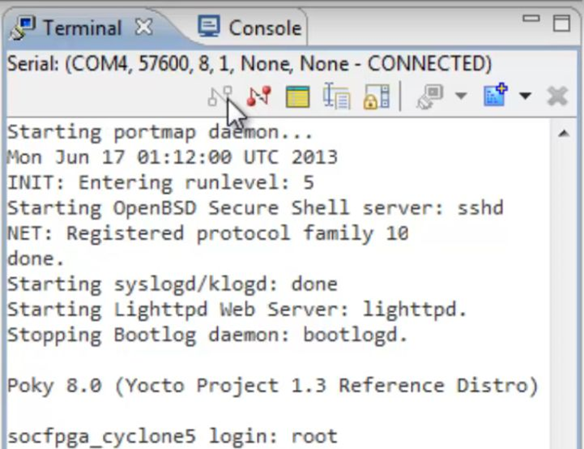
\includegraphics[width=0.8\textwidth]{img/debugterminal}
	\caption{Debug terminal}
    	\label{fig:debugterminal}
\end{figure}

To debug on Linux with the Cyclone V was needed an Eclipse based environment called DS-5 debugger included in the intelFPGA software.\\
We connected it to the serial and the boot was showed in its terminal panel.
\clearpage

\begin{figure}[h]
	\centering		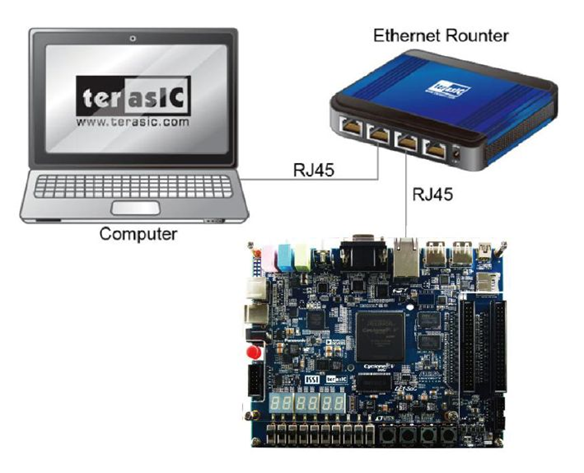
\includegraphics[width=0.8\textwidth]{img/routerconf}
	\caption{Router connection}
    	\label{fig:routerconf}
\end{figure}

As told in “My First HPS guide provided by Altera, a router was needed to connect the PC with the board via Ethernet.\\
However the router was only needed for its DHCP protocol, so we manually configured the board with ifconfig eth0 $192.168.1.4$ netmask $255.255.255.0$ up in the terminal.\\
In Windows in LAN settings we configured the network as in the image.\\
We executed the ping command and it worked.
\clearpage

\begin{figure}[h]
	\centering		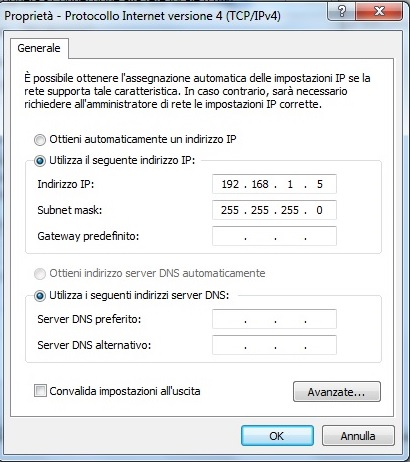
\includegraphics[width=0.6\textwidth]{img/internetprop}
	\caption{Internet properties}
    	\label{fig:internetprop}
\end{figure}

\begin{figure}[h]
	\centering		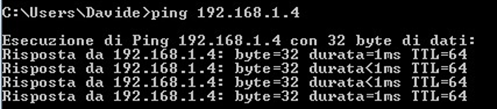
\includegraphics[width=0.8\textwidth]{img/ping}
	\caption{Connection test}
    	\label{fig:ping}
\end{figure}

\clearpage
We executed the following commands to activate the ssh protocol.\\
Then in the remote system panel  we defined an ssh only connection with host name the board IP and a connection name. We opened it and it requested a password, but was only necessary to write root in the host name to gain the access.\\

\begin{figure}[h]
	\centering		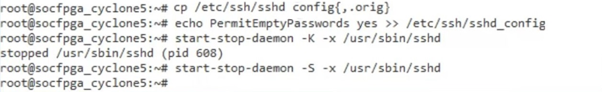
\includegraphics[width=0.6\textwidth]{img/comand}
	\caption{Commands}
    	\label{fig:comand}
\end{figure}


Once established a connection to test the debug function, we opened a software made by Altera: intelFPGA-embedded-examples-software-Altera-SoCFPGA-Blinking-LED-Linux-GNU.tar.gz\\
When we tried to build the project an error showed up due to a licensing problem:


\begin{figure}[h]
	\centering		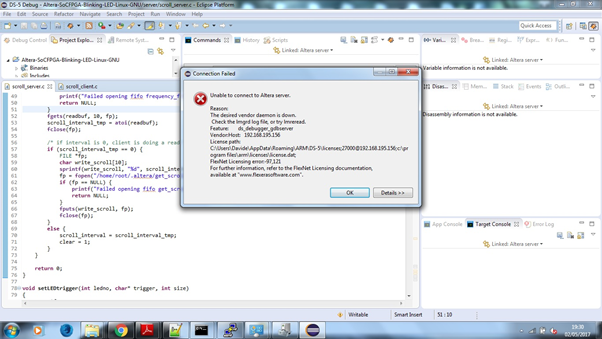
\includegraphics[width=0.8\textwidth]{img/licenseerror}
	\caption{License error}
    	\label{fig:licenseerror}
\end{figure}

Once downloaded the licence, it builded the project. Then we created a new configuration in the panel “Debug configuration” for the application server side following these steps:

\clearpage
\begin{figure}[h]
	\centering		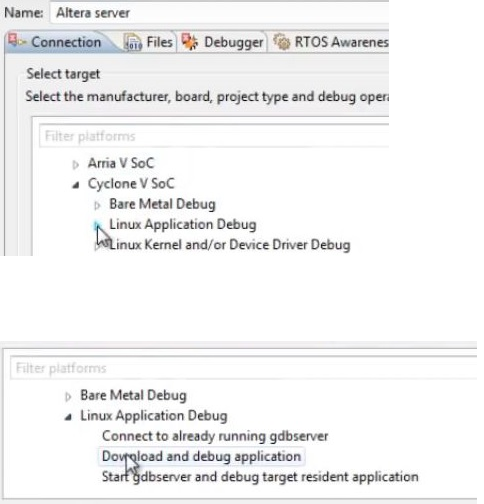
\includegraphics[width=0.8\textwidth]{img/downloadonborad}
	\caption{Download on borad}
    	\label{fig:downloadonborad}
\end{figure}

\begin{figure}[h]
	\centering		
\includegraphics[width=0.8\textwidth]{img/downloadsucces}
	\caption{Download success}
    	\label{fig:downloadsucces}
\end{figure}

Same steps for the client side but changing the following parameters.


\begin{figure}[h]
	\centering		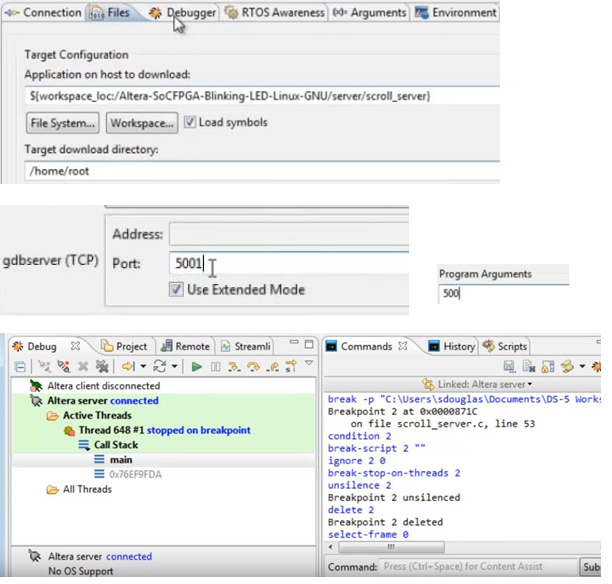
\includegraphics[width=0.8\textwidth]{img/setting}
	\caption{Settings}
    	\label{fig:setting}
\end{figure}

Click on Altera server and start debug.

\begin{figure}[h]
	\centering		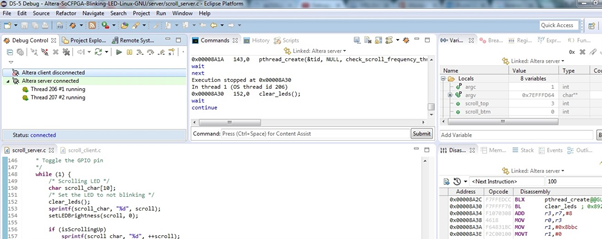
\includegraphics[width=0.8\textwidth]{img/debug}
	\caption{Debug}
    	\label{fig:debug}
\end{figure}
















\chapter{Conclusions}

\label{ch:conclusions}
La mobilità delle persone e delle merci sono una componente essenziale del mercato interno dell'Unione Europea (UE) ed è di fondamentale importanza garantire la sua fattibilità al fine di salvaguardare la crescita economica.
La rete ferroviaria ha un ruolo strategico in questo contesto almeno sotto due punti di vista:

\cleardoublepage

%----------------------------------------------------------------------------------------
%	Appendici della relazione
%----------------------------------------------------------------------------------------

\appendix

\part{Appendix}

\chapter{Online question}

\section{VxWorks question}

\section{BlaBla question}


%----------------------------------------------------------------------------------------
%	Bibliografia
%----------------------------------------------------------------------------------------

\cleardoublepage% Bibliography
\label{app:bibliography}

\manualmark
\markboth{\spacedlowsmallcaps{\bibname}}{\spacedlowsmallcaps{\bibname}} % Work-around to have small caps also
%\phantomsection
\refstepcounter{dummy}

\addtocontents{toc}{\protect\vspace{\beforebibskip}} % Place the bibliography slightly below the rest of the document content in the table of contents
\addcontentsline{toc}{chapter}{\tocEntry{\bibname}}

\printbibliography

\begin{itemize}
\begin{sloppypar}
\item \url{https://www.altera.com/products/fpga/cyclone-series/cyclone-v/overview.html}
\item \url{https://knowledge.windriver.com/en-us/000_Products/000/020/010/000}
\item \url{http://www.terasic.com.tw/cgi-bin/page/archive.pl?Language=English&No=836&PartNo=4}
\item \url{http://dl.altera.com/16.1/?edition=standard}
\item \url{https://support.dce.felk.cvut.cz/psr/cviceni/target/}
\item \url{https://dl.altera.com/soceds/}
\item \url{https://www.altera.com/support/support-resources/download/rtos_tools.html}
\item \url{https://marketplace.windriver.com/index.php?bsp&on=details&bsp=12660}
\item \url{https://www.windriver.com/licensing/documents/wr_product_install_licensing_developers_guide_2.6.pdf}
\item \url{https://www.xilinx.com/support/documentation/application_notes/xapp1114.pdf}
\item \url{https://knowledge.windriver.com/@api/deki/files/241699/vxworks_bsp_developers_guide_6.9.pdf}
\item \url{https://rocketboards.org/foswiki/view/Documentation/PreloaderUbootCustomization131#HPS_Boot_Flow}
\item \url{https://rocketboards.org/foswiki/view/Documentation/WebHome}
\item \url{https://www.altera.com/content/dam/altera-www/global/en_US/pdfs/literature/hb/cyclone-v/cv_5400a.pdf}
\item \url{http://zedboard.org/sites/default/files/documentations/GS-AES-Z7EV-7Z020-G-V7.pdf}
\item \url{http://zedboard.org/sites/default/files/documentations/CY7C64225_Setup_Guide_1_3.pdf}
\item \url{http://zedboard.org/sites/default/files/documentations/ZedBoard_HW_UG_v2_2.pdf}
\item \url{https://www.xilinx.com/support/documentation/application_notes/xapp1158-zynq-7000-vxworks-bsp.pdf}
\item \url{https://www.xilinx.com/support/documentation/sw_manuals/xilinx2014_1/ug1043-embedded-system-tools.pdf}
\item \url{http://www.wiki.xilinx.com/Prepare+boot+image}
\item \url{https://forums.xilinx.com/t5/Embedded-Development-Tools/AP-transaction-Error/td-p/369465}
\end{sloppypar}
\end{itemize}

 % Bibliography


%----------------------------------------------------------------------------------------

\end{document}
